% Copyright (c) 2023 Ignacio Slater Muñoz All rights reserved.
% Use of this source code is governed by a BSD-style
% license that can be found in the LICENSE file.

\begin{definition}[Position Based Crossover]
    The \textit{position based crossover} operator works with two input chromosomes. It strategically copies certain 
    positions from one input, while the rest of the genes are filled in from the other input without duplicating any 
    genes. Formally, the position based crossover is illustrated as:

    \begin{equation}
        X_\mathrm{pbx}(P: \mathbb{P},\, \rho_\textbf{i}: [0,\, 1],\, \rho_\mathbf{c}: [0,\, 1]) \to \mathbb{P}
    \end{equation}

    where:

    \begin{itemize}
      \item \(P\) signifies a population of ordered chromosomes.
      \item \(\rho_\textbf{i}\) denotes the probability of utilizing the crossover for an individual.
      \item \(\rho_\mathbf{c}\) signifies the likelihood of adopting the position based crossover for a chromosome.
    \end{itemize}
\end{definition}

The way PBX is implemented in the \textit{Keen} framework is as follows:

\begin{code}{
    PBX algorithm as executed in the \textit{Keen} framework. For simplicity, we represent chromosomes as arrays,
    meaning that \texttt{output1[i] = input1[i]} signifies that the \texttt{i}-th gene in \texttt{output1} will be
    assigned the value of the \texttt{i}-th gene in \texttt{input1}. \texttt{input1} and \texttt{input2} are the parent
    chromosomes, while \texttt{output1} and \texttt{output2} are the offspring chromosomes. All arrays are assumed to
    be of the same size.
}{
    label={lst:keen:op:cx:pbx}
}{kotlin}
    val positions = random.indices in input1
    val output = input1
    for (i in positions) {
        output[i] = input1[i]
    }
    var j = 0
    for (i in 0..input2.size) {
        if (input2[i] not in output) {
            output[positions[j++]] = input2[i]
            if (j >= positions.size) {
                break
            }
        }
    }
    return output
\end{code}

In the PBX method, select positions from the first input chromosome are directly copied to the output. The remaining 
genes from the second input chromosome are then filled in the order they appear, skipping any that are already present 
in the output. A visual representation of this process can be seen in \vref{fig:keen:op:cx:pbx}

\begin{figure}[ht!]
\centering
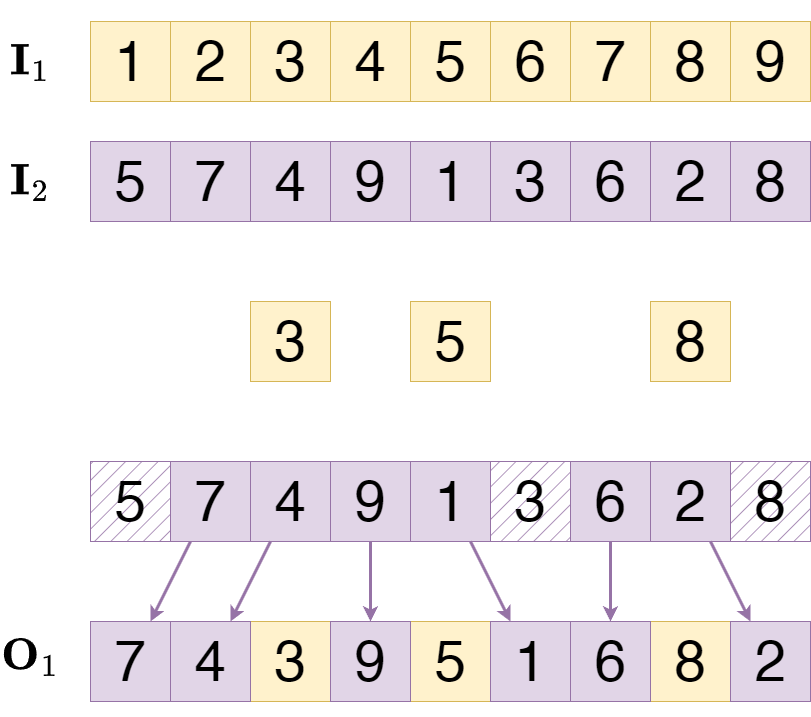
\includegraphics[width=0.33\textwidth]{img/keen/PBX.png}
\caption{Position Based Crossover (PBX) operation.}
\label{fig:keen:op:cx:pbx}
\end{figure}
